\documentclass[12pt,letterpaper,noanswers]{exam}
\usepackage[usenames,dvipsnames,svgnames,table]{xcolor}
\usepackage[margin=0.9in]{geometry}
\renewcommand{\familydefault}{\sfdefault}
\usepackage{multicol}
\pagestyle{head}
\header{AM 111 Class 09}{}{Interpolation, p.\thepage}
\runningheadrule
\headrule
\usepackage{siunitx}
\usepackage{graphicx} % more modern
\usepackage{amsmath} 
\usepackage{amssymb} 
\usepackage{hyperref}
\usepackage{tcolorbox}
\usepackage{enumitem}
\def\mbf{\mathbf}
\newcommand{\vc}[1]{\boldsymbol{#1}}
\def\dsst{\displaystyle}
\DeclareMathOperator*{\argmin}{arg\,min} % thin space, limits underneath in displays


\begin{document}
 \pdfpageheight 11in 
  \pdfpagewidth 8.5in

\noindent 

\section*{Preliminaries}

\begin{itemize}
\itemsep0pt
\item Problem set 04 is due on Friday at noon.
\item There will be a skill check in class during Class 09.  The problem info is below.
\item Find all OH on Canvas.
\item Quiz 01 is on Thursday Oct 12.  There is quiz info on canvas.
\end{itemize}



\noindent\textbf{Big picture}

Today: Algorithms for finding a curve that directly passes through data points.

\vspace{0.2cm}
\hrule
\vspace{0.2cm}

\noindent \textbf{Skill check practice}
 Consider the data points $(1,7)$, $(3, 5)$, $(4, 9)$.  Construct $L_{3,1}$, the Lagrange basis function of degree $2$ that is $1$ at $x_1 = 1$ and is $0$ at the other input values.



\vspace{0.2cm}
\hrule
\vspace{0.2cm}

\noindent \textbf{Skill check solution}
For zeros at $3$ and $4$, we have $(x-3)(x-4)$.  For the function to be $1$ at $x = 1$, we have $L_{3,1} = \dfrac{(x-3)(x-4)}{(1-3)(1-4)}$

\vspace{0.2cm}
\hrule
\vspace{0.2cm}


\section*{Interpolation}
\subsection*{Some applications}
\begin{multicols}{2}
\begin{itemize}
\itemsep0pt
    \item rendering fonts
    \item approximated a complicated function by a polynomial
    \item numerical integration
    \item creating a smooth surface given data
    \item design and manufacturing (aircraft, cars)
    \item animation / graphics
    \item spline smoothing methods
\end{itemize}
\end{multicols}

\subsection*{Numerical integration}

Methods for numerical integration (also called quadrature) will be based on finding low-degree polynomial approximations to the function we would like to integrate.

Instead of integrating the function, we integrate the low-degree polynomial approximation.

Example: trapezoid rule.  Fit a linear function to every successive pair of data points and integrate those linear functions.

Example: simpson's rule.  Fit a quadratic function to every set of three data points and integrate those quadratic functions.

As part of our integration work, we will want to understand the error associated with the polynomial fit.


\subsection*{Polynomial interpolation of data}
\begin{tcolorbox}
(Sauer \S3.1)

A function $y = P(x)$ \textbf{interpolates} the data points $\{(x_i,y_i)\}_{i=1}^n$ if $P(x_i) = y_i$ for $1\leq i\leq n$.
\end{tcolorbox}
\begin{enumerate}[resume=classQ]
\item Consider the data points $(0,3), (1,2), (2,4)$.  What is the lowest degree polynomial that will interpolate these points?
\vspace{0.6in}

\item Consider the data points $(0,3), (0,2), (2,4)$.  Is an interpolating function possible?  Why not?
\vspace{0.6in}

\end{enumerate}

\subsection*{Monomial basis}
\begin{tcolorbox}
For $N$ data points, choose $N$ basis functions, $1$, $x$, ..., $x^k$,..., $x^{N-1}$.
Set up a linear system (similar to least squares):
\[\left[\begin{array}{c c c c}
1 & x_1 & \hdots & x_1^{N-1} \\
\vdots & \vdots & & \vdots \\
1 & x_N & \hdots & x_N^{N-1}
\end{array}\right]
\left[\begin{array}{c}
w_1 \\
w_2 \\
\vdots \\
w_N
\end{array}\right] = 
\left[\begin{array}{c}
y_1 \\
y_2 \\
\vdots \\
y_N
\end{array}\right]\]
\end{tcolorbox}
\begin{enumerate}[resume=classQ]
\item Recall that the matrix \[\left[\begin{array}{c c c c}
1 & x_1 & \hdots & x_1^{N-1} \\
\vdots & \vdots & & \vdots \\
1 & x_N & \hdots & x_N^{N-1}
\end{array}\right]\] is called a \textbf{Vandermonde} matrix.  

\emph{You worked with Vandermonde matrices on problem set 02.} 

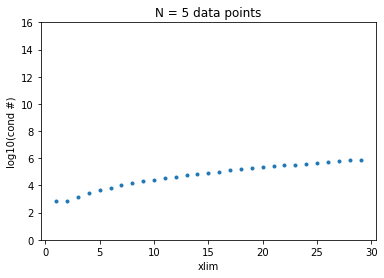
\includegraphics[width=0.45\textwidth]{img/Class08vandermonde5.png}
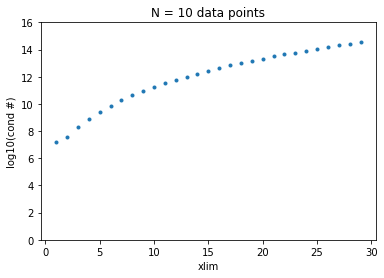
\includegraphics[width=0.45\textwidth]{img/Class08vandermonde10.png}

\begin{verbatim}
N = 5
xlim = 8
xlist = np.linspace(0,xlim,N)
A = np.vander(xlist)
condnum = np.linalg.cond(A)
\end{verbatim}

What makes the basis $1$, $x$, ..., $x^k$,..., $x^{N-1}$ a poor choice for finding an interpolating polynomial?
\vspace{1in}
\end{enumerate}

\begin{tcolorbox}
\begin{itemize}
\itemsep0pt
    \item (From Heath \S 7.3.1)
    
    Solving the system $A\vc{c} = \vc{y}$ to determine $\vc{c}$, where $A$ is the Vandermonde matrix , requires $\mathcal{O}(n^3)$ work.
    \item (from Heath \S Notation)
    
    $\mathcal{O}(n^3)$ is ``big-oh'' notation.  For $n$ large, $f(n) = \mathcal{O}(g(n))$ (said ``$f$ is of the order $g$'' or ``$f$ is big-oh of $g$'' if there is a $C>0$ such that $\vert f(n)\vert \leq C\vert g(n)\vert$ for all $n$ sufficiently large.  For example, $7n^3 + 2n^2 + n = \mathcal{O}(n^3)$.
    
    \item `$\mathcal{O}(n^3)$ work' refers to the number of multiplications required to carry out the algorithm.
\end{itemize}
\end{tcolorbox}

\noindent\textbf{Advantages of the monomial basis}
\begin{tcolorbox}
(From Heath \S 7.3.1)
\begin{itemize}
\itemsep0pt
    \item 
    
    The polynomial can be evaluated in $n$ additions and $n$ multiplications.
    
    \item differentiation and integration are also straightforward
   
\end{itemize}

\end{tcolorbox}

\subsection*{Lagrange interpolation}
\emph{(questions from Veronica Ciocanel)}
\begin{enumerate}[resume=classQ]

\item Given two distinct points $(x_0,y_0)$ and $(x_1,y_1)$, find an equation for the
straight line through both points. 

Call this function $P(x)$.  Is it unique?

\emph{A line is the lowest dimensional interpolating polynomial for two points.}

\vspace{1in}

\item Show that the function $\dsst{L_0(x) = \frac{x-x_1}{x_0-x_1}}$ is $1$
when $x=x_0$ and $0$ when $x=x_1$.  

Similarly $\dsst{L_1(x) = \frac{x-x_0}{x_1-x_0}}$
is $0$ when $x=x_0$ and $1$ when $x=x_1$.

\vspace{1in}

\item Consider the function $Q(x) = y_0L_0(x) + y_1L_1(x)$.  Show that it is
equal to $P(x)$.

\vspace{1in}

\end{enumerate}

\begin{tcolorbox}
\begin{itemize}
\itemsep0pt
\item (Lagrange interpolation)
Let $(x_1,y_1),...,(x_n,y_n)$ be $n$ points in the plane with distinct $x_k$.  There exists a polynomial $P(x)$ of degree at most $n-1$
with $P(x_k) = y_k$ for all $k$.

This polynomial is given by 
\[
P(x) = y_1L_{n,1}(x) + \cdots y_n L_{n,n}(x) = \sum_{k=1}^n y_k L_{n,k}(x)
\]
where, for each $k=1,...,n$
\[
L_{n,k} = \frac{(x-x_1)(x-x_2)\cdots(x-x_{k-1})(x-x_{k+1})\cdots(x-x_n)}
{(x_k-x_1)(x_k-x_2)\cdots(x_k-x_{k-1})(x_k-x_{k+1})\cdots(x_k-x_n)}
=\prod_{i\ne k} \frac{x-x_i}{x_k-x_i}
\]

The $L_{n,k}$ are the \textbf{Lagrange basis functions} for $\mathcal{P}_{n-1}$ (the space of polynomials of degree $n-1$).  They can also be called \textbf{fundamental polynomials} or \textbf{cardinal functions}.  (Heath \S 7.3.2)

\item (Sauer \S 3.1.1 Theorem 3.2: uniqueness of $P$) 
Let $(x_1,y_1),...,(x_n,y_n)$ be $n$ points in the plane with distinct $x_k$.  There exists one, and only one, polynomial $P(x)$ of degree at most $n-1$
with $P(x_k) = y_k$ for all $k$.

%\item It requires $\mathcal{O}(n^2)$ arithmetic operations to find $P(x)$, and evaluation requires $\mathcal{O}(n)$.

%\item To add a new data point and construct a new interpolating polynomial can be done in $\mathcal{O}(n)$ operations.
\end{itemize}

 
\end{tcolorbox}

\begin{enumerate}[resume=classQ]

\item Construct the Lagrange interpolating polynomial that goes through the points $(0,1)$, $(2,2)$, and $(3,4)$.  %Simplify it to the form $P(x) = ax^2 + bx + c$.

\vspace{1in}

\item Consider the Lagrange interpolation problem.  If it is written in the form $A\vc{c} = \vc{y}$ (where $\mathbf{c}$ are the weights assigned to the basis functions), what is the structure of $A$?

\emph{Use your knowledge of the values of the weights, $\vc{c}$.}
\vspace{0.5in}
\end{enumerate}

\subsection*{Summary}
Using the Lagrange basis leads to a diagonal $A$.  

%Another basis that is sometimes used (Newton basis functions) leads to a triangular $A$.

\subsection*{Newton's divided differences}
\begin{tcolorbox}
\begin{itemize}
    \item The basis functions are $\pi_j(x) = \prod\limits_{k = 1}^{j-1}(x-x_k),\quad j = 1,...,n$
    \item $A$ is lower triangular: $\pi_j(x_i) = 0$ for $i<j$.  The solution can be found in $\mathcal{O}(n^2)$ operations.
    \item Nested evaluation: $P_{n-1}(x) = c_1 + (x-x_1)(c_2 + (x-x_2)(c_3+ (x-x_3)(...(c_{n-1} + c_n(x-x_{n-1}))...)))$
    \item Adding a new point, $P_j(x) = P_{j-1}(x) + c_j\pi_j(x)$ and $P_j(x_j) = y_j$ so $c_j = \dfrac{y_j - P_{j-1}(x_{j})}{\pi_j(x_j)}$
    \item The divided differences method of finding $c_j$ has better numerical properties that using direct formulation of the matrix and using forward substitution to solve.
    \item Newton interpolation does not depend on a particular ordering of the points.  Conditioning of $A$ does vary with the order of the points, though. 

\end{itemize}
    
\end{tcolorbox}


\begin{enumerate}[resume]
\item For $(0,1), (2,3)$ construct $A\mathbf{c} = \mathbf{y}$ or the divided difference table.



Let $P_1(x) = c_0 + c_1(x-0)$.  Find $c_0$ and $c_1$.

Check $P_1(0)$ and $P_1(2)$.

\item Add the third data point $(3,0)$.

$P(x) = c_0 + c_1(x-0) + c_2(x-0)(x-2)$.  Find $c_0$, $c_1$, $c_2$.

Check $P(0), P(2)$, and $P(3)$.
\end{enumerate}

% \section*{Piecewise polynomial interpolation (splines)}

% (Koumoutsakos et al lecture 4)

% Using a high degree polynomial to interpolate data (as happens in the problems above when $N$ is larger), means the polynomial is likely to be highly oscillatory.  The polynomial may not look like the function being approximated from the sample points.

% 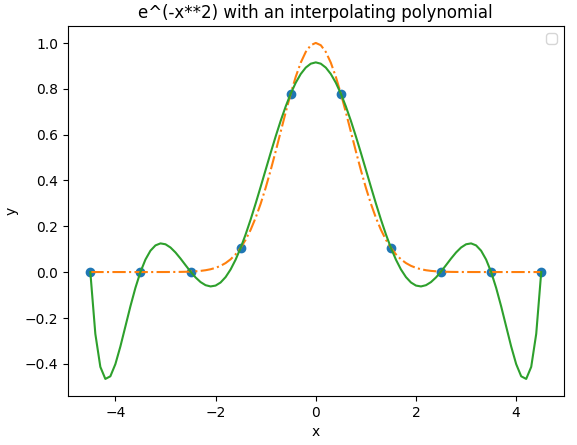
\includegraphics[width=0.7\textwidth]{img/C08gaussinterp.png}

% \begin{tcolorbox}
% Fit a polynomial to the data piecewise (using just a few data points at a time).
% \end{tcolorbox}

% 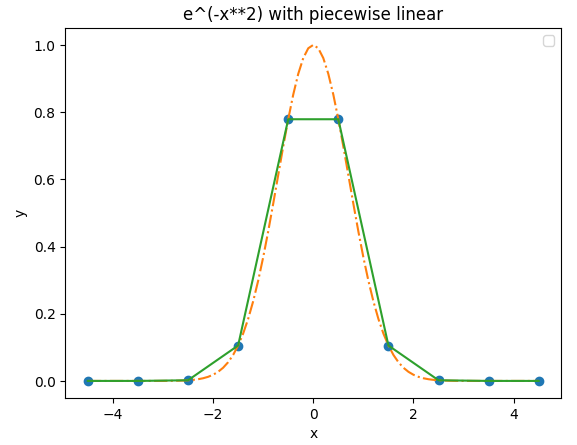
\includegraphics[width=0.7\textwidth]{img/C08linearpiece.png}

% 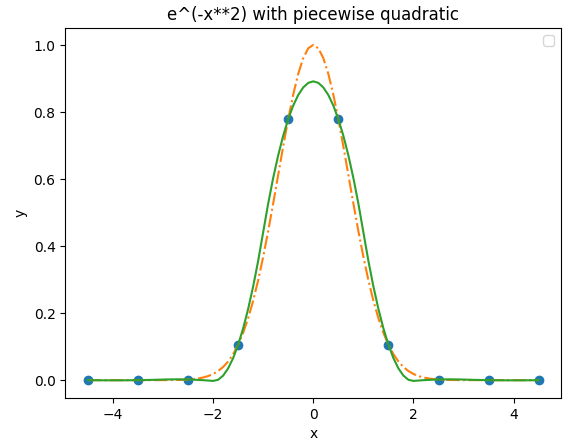
\includegraphics[width=0.7\textwidth]{img/C08picequad.png}

\end{document}